%%
%  ******************************************************************************
%  * #file    Szablon_raportu_EN_Latex.tex
%  * #author  Adrian Wójcik   adrian.wojcik(at)put.poznan.pl
%  *          
%  * #commit  Patryk Kościk   koscikpatryk(at)gmail.com
%  *          Modified the template for Projekt przejsciowy purposes          
%  *          
%  *
%  * #commit  Patryk Kościk   koscikpatryk(at)gmail.com
%  *          Zupełnie przewrócono na łeb formatke po taktycznym wyjasnieniu          
%  *          
%  * #version 1.1
%  * #date    09-Mar-2022
%  * #brief   PROJPRZEJ
%  *
%  ******************************************************************************
%%  
\documentclass[11pt, a4paper]{article}

\usepackage{SM_template}

% Wypełnijcie te dyrektywy zgodnie z waszym tematem
%
% \lab      -> NAZWA CZUJNIKA,          np.: 'DHT22'
% \comment  -> Króciutki opis co to,    np.: 'Cyfrowy czujnik temperatury'
% \author   -> Autor dokumentu          np.: Patryk Kościk
%
% Pamiętajcie o zmianie ścieżki w \addbibresourcue (!)

\lab{Moduł TC77}
\comment{Cyfrowy czujnik temperatury}
\author{Jakub Grzesiak}
\addbibresource{bib/TC77.bib}

%
% Początek dokumentu
%
\begin{document}

%
% Strona tytułowa
%
\mainpage{TC77/zdj_modułu/front.jpg}
\newpage

\section*{Opis elementu}
Cyfrowy czujnik temperatury TC77 (ang. thermal sensor) to sensor zawierający diodę termiczną, 13-bitowy konwerter analogowo-cyfrowy (dokładnie 12-bitowy z dodatkowym bitem znaku), rejestr temperatury (TRM) odpowiedzialny za zapisanie ostatnio zmierzonej temperatury, rejestr identyfikacyjny producenta, rejestr konfiguracyjny oraz interfejs portu szeregowego odpowiedzialny za komunikację poprzez protokoły SPI i MICROWIRE. Budowa całego czujnika została przedstawiona na diagramie blokowym (\ref{fig:_zasada_dzialania_elementu}). Czujniki TC77, dzięki swojemu małemu rozmiarowi i niskim poborze prądu rzędu setek $\mu A$, znajdują zastosowanie w telefonach komórkowych, dyskach twardych, sterowaniu przemysłowym czy jako zamienniki termistorów.


%%%%%%%%%%%%%%%%%%%%%%%%%  TWO IMAGES SIDE BY SIDE  %%%%%%%%%%%%%%%%%%%%%%%%%%%%%
\vspace{0.25cm}
\begin{figure}[h]
\centering
%%%%%%%%%%%%%%%%%%%%%%%%%%%%%%%%%%%%%%%%%%%%%%%%%%%%%%%%%%%%%%%%%%%%%%%%%%%%%%%%%
\begin{subfigure}{.5\textwidth}
\centering
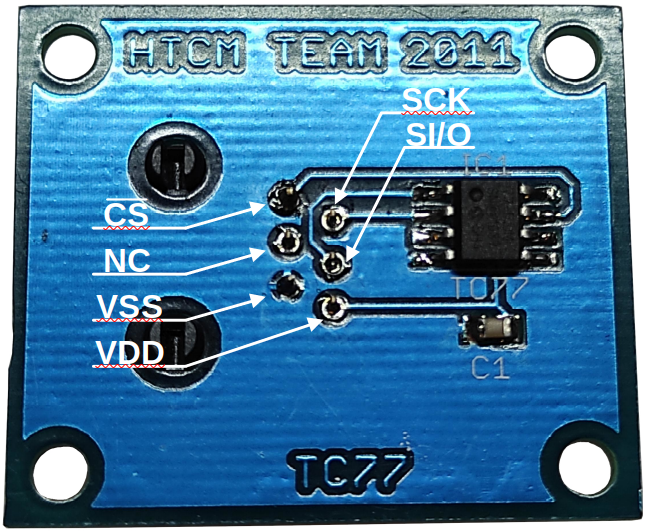
\includegraphics[width=.7\linewidth]{fig/TC77/zdj_modułu/TC77_oznaczenie.png}
\caption{Fizyczna budowa modułu wraz z pinoutem}
\label{fig:_zdjecie_elementu}
\end{subfigure}%
%%%%%%%%%%%%%%%%%%%%%%%%%%%%%%%%%%%%%%%%%%%%%%%%%%%%%%%%%%%%%%%%%%%%%%%%%%%%%%%%%
\begin{subfigure}{.5\textwidth}
\centering
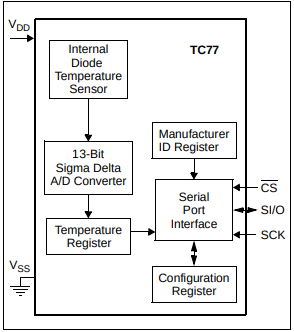
\includegraphics[width=0.8\linewidth]{fig/TC77/zdj_modułu/block_diagram.png}
\caption{Diagram blokowy budowy czujnika \cite{microchip:TC77}}
\label{fig:_zasada_dzialania_elementu}
\end{subfigure}
%%%%%%%%%%%%%%%%%%%%%%%%%%%%%%%%%%%%%%%%%%%%%%%%%%%%%%%%%%%%%%%%%%%%%%%%%%%%%%%%%
% \caption{PODPIS}
\label{fig:element}
\end{figure}
\vspace{0.25cm}
%%%%%%%%%%%%%%%%%%%%%%%%%  TWO IMAGES SIDE BY SIDE  %%%%%%%%%%%%%%%%%%%%%%%%%%%%%
Moduł może być zasilany napięciami z zakresu $2,7V - 5,5V DC$. Schemat elektryczny budowy wewnętrznej przedstawiono na rysunku (\ref{fig:_schemat_modulu}). Kondensator C1 pełni rolę filtra napięcia zasilającego $V_{DD}$. \\ \\
Pomiar temperatury za pomocą diody termicznej opiera się liniowej zależności napięcia i do temperatury - wraz ze wzrostem temperatury maleje napięcie przewodzenia. Minimalna i maksymalna temperatura, jaką czujnik może wykryć to odpowiednio $-55 ^\circ C$ i $+125 ^\circ C$. Rozdzielczość wynosi $0,0625 ^\circ C$.
%%%%%%%%%%%%%%%%%%%%%%%%%  TWO IMAGES SIDE BY SIDE  %%%%%%%%%%%%%%%%%%%%%%%%%%%%%
\begin{figure}[h]
\centering
%%%%%%%%%%%%%%%%%%%%%%%%%%%%%%%%%%%%%%%%%%%%%%%%%%%%%%%%%%%%%%%%%%%%%%%%%%%%%%%%%
\begin{subfigure}{.5\textwidth}
\centering
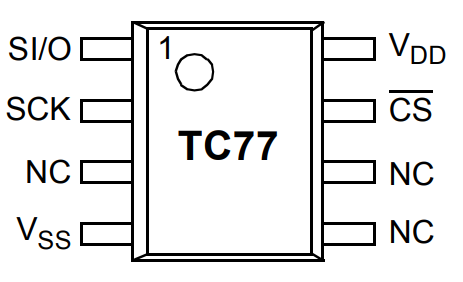
\includegraphics[width=.8\linewidth]{fig/TC77/zdj_modułu/schem_datasheet.png}
\caption{Przedstawienie wyprowadzeń w obudowie SOIC \cite{microchip:TC77}}
\label{fig:_zdjecie_modulu}
\end{subfigure}%
%%%%%%%%%%%%%%%%%%%%%%%%%%%%%%%%%%%%%%%%%%%%%%%%%%%%%%%%%%%%%%%%%%%%%%%%%%%%%%%%%
\begin{subfigure}{.5\textwidth}
\centering
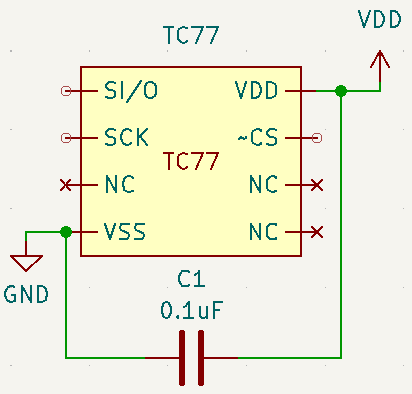
\includegraphics[width=.55\linewidth]{fig/TC77/polaczenie_modulu/schemat_kicad.png}
\caption{Schemat budowy wewnętrznej modułu}
\label{fig:_schemat_modulu}
\end{subfigure}
%%%%%%%%%%%%%%%%%%%%%%%%%%%%%%%%%%%%%%%%%%%%%%%%%%%%%%%%%%%%%%%%%%%%%%%%%%%%%%%%%
\label{fig:modul}
\end{figure}
\vspace{0.25cm}
%%%%%%%%%%%%%%%%%%%%%%%%%  TWO IMAGES SIDE BY SIDE  %%%%%%%%%%%%%%%%%%%%%%%%%%%%%

% \subsection{Opis modułu} REPLACE SUBSECTION WITH 1CM VSPACE
Protokół komunikacyjny SPI (ang. Serial Peripheral Interface) jest protokołem synchronicznym typu master-slave. Oznacza to, że w jednej chwili tylko jeden układ może prowadzić komunikację z odbiorcą. Na zdjęciu (\ref{fig:_zdjecie_elementu}) oznaczono wszystkie wyjścia magistrali interfejsu SPI oraz zasilania wyprowadzone na płytkę PCB, odpowiednio: 
\begin{itemize}
  \item $\overline{CS}$ - Chip Select - aktywacja danego układu, z którym zestawiana będzie komunikacja
  \item $SCK$ - Serial Clock - taktowanie zegara (interfejs synchroniczny)
  \item $NC$ - Not Connected - pin niepodłączony
  \item $SI/O$ - Serial Data (Input/Output) - szeregowy pin do przesyłu danych
  \item $VSS$ - pin masy
  \item $VDD$ - pin zasilania
\end{itemize}

Ramka danych odbieranych z czujnika przez protokół SPI to 2-bajtowe słowo (16 bitów). Do odczytu temperatury używane jest jednak tylko 13 bitów. Najbardziej znaczący bit - MSB (ang. Most Significant Bit) wskazuje znak temperatury (dodatnia - '0', ujemna - '1'). Na rysunku (\ref{fig:_frame}) przedstawiającym ramkę danych zawierających temperaturę pominięto 3 najmniej znaczące bity nieniosące ważnych informacji. Odczyt danych na linii SI/O synchronizowany jest zboczem narastającym sygnału zegarowego $SCK$, którego częstotlwiość nie może przekraczać $7MHz$ \cite{microchip:TC77}. Transmisja rozpoczyna się, gdy linia $\overline{CS}$ przyjmuje stan niski.

\vspace{0.25cm}
\begin{figure}[h]
    \centering
    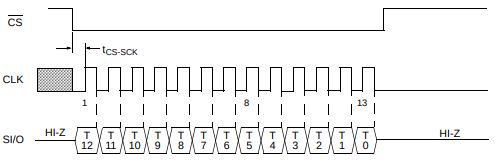
\includegraphics[width=0.8\textwidth]{fig/TC77/zasada_dzialania/frame.png}
    \caption{Ramka SPI zawierająca dane o temperaturze \cite{microchip:TC77}}
    \label{fig:_frame}
\end{figure}
\vspace{0.25cm}

\newpage
\section{Użycie czujnika}
Czujnik posiada 3 wyprowadzenia interfejsu SPI ($SI/O, SCK$ i $\overline{CS}$) oraz 2 wyprowadzenia zasilające. Na rys. \ref{fig:_zdjecie_elementu} przedstawiono oznaczenia wyprowadzeń rzeczywistego czujnika. Działanie czujnika można zweryfikować z użyciem mikrokontrolera. W poniższym przykładzie użyto płytki rozwojowej STM32 NUCLEO-F767ZI. Układ połączeń przedstawiony na rysunku (\ref{fig:_polaczenie_ukladu}) oraz program dla płytki NUCLEO-F746ZG będzie identyczny. Kod skonfigurowano tak, aby przez komunikację szeregową UART wysyłana była co $0,5s$ aktualna wartość temperatury odczytana z czujnika. Dodatkowo, działanie programu fizycznie sygnalizuje miganie niebieskiej, wbudowanej w płytkę diody LD2.

\vspace{0.25cm}
\begin{figure}[h]
    \centering
    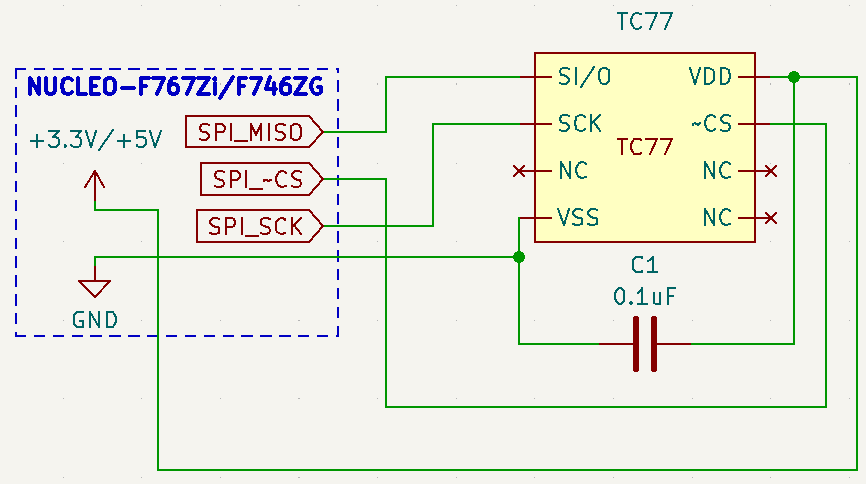
\includegraphics[width=0.7\textwidth]{fig/TC77/polaczenie_modulu/nucleo_con.png}
    \caption{Połączenie układu z mikroprocesorem}
    \label{fig:_polaczenie_ukladu}
\end{figure}
\vspace{0.25cm}

Poniżej zaprezentowano zdjęcie rzeczywistego układu oraz jego przykładowe odpowiedzi z temperaturą wysyłane poprzez UART. Konfiguracja pliku \texttt{.IOC} i kod zawarte są w \texttt{Suplement \#1}.

% TUTAJ FOTY ODNOSNIE TEGO
%%%%%%%%%%%%%%%%%%%%%%%%%  TWO IMAGES SIDE BY SIDE  %%%%%%%%%%%%%%%%%%%%%%%%%%%%%
\vspace{0.25cm}
\begin{figure}[h]
\centering
%%%%%%%%%%%%%%%%%%%%%%%%%%%%%%%%%%%%%%%%%%%%%%%%%%%%%%%%%%%%%%%%%%%%%%%%%%%%%%%%%
\begin{subfigure}{.5\textwidth}
\centering
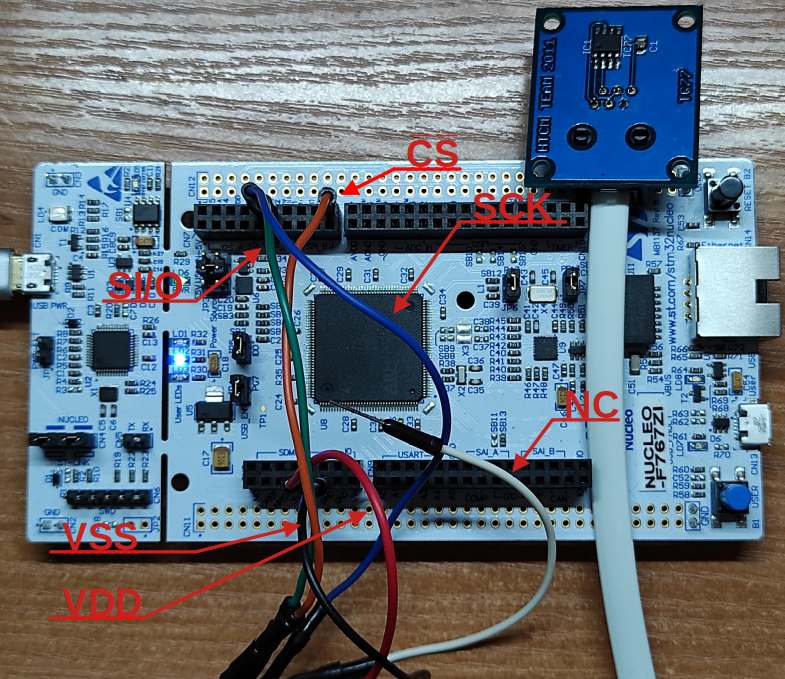
\includegraphics[width=1\linewidth]{fig/TC77/polaczenie_modulu/board.png}
\caption{Fizyczne połączenie układu z mikroprocesorem}
\label{fig:_board}
\end{subfigure}%
%%%%%%%%%%%%%%%%%%%%%%%%%%%%%%%%%%%%%%%%%%%%%%%%%%%%%%%%%%%%%%%%%%%%%%%%%%%%%%%%%
\begin{subfigure}{.5\textwidth}
\centering
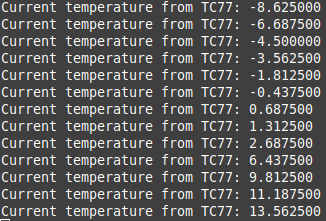
\includegraphics[width=0.9\linewidth]{fig/TC77/polaczenie_modulu/uart.png}
\caption{Przykładowe odczyty temperatury}
\label{fig:_uart}
\end{subfigure}
%%%%%%%%%%%%%%%%%%%%%%%%%%%%%%%%%%%%%%%%%%%%%%%%%%%%%%%%%%%%%%%%%%%%%%%%%%%%%%%%%
% \caption{PODPIS}
\label{fig:mikroproc}
\end{figure}
\vspace{0.25cm}
%%%%%%%%%%%%%%%%%%%%%%%%%  TWO IMAGES SIDE BY SIDE  %%%%%%%%%%%%%%%%%%%%%%%%%%%%%
Dodatkowo działanie układu przedstawiono na załączonym w \texttt{Suplement Wideo} materiale 
wideo.

\newpage
\printbibliography[heading=bibintoc]

\end{document}